%!TEX root = main.tex
%!TEX program = lualatex
%%%% Define Article %%%%%%%%%%%%%%%
\documentclass[
  a4paper,
  12pt
]{article}
%%%%%%%%%%%%%%%%%%%%%%%%%%%%%%%%%%%


%%%% Using Packages %%%%%%%%%%%%%%%
\usepackage{geometry}
\usepackage{graphicx}
\usepackage{amssymb}
\usepackage{amsmath}
\usepackage{amsthm}
\usepackage{empheq}
\usepackage{mdframed}
\usepackage{booktabs}
\usepackage{lipsum}
\usepackage{graphicx}
\usepackage{color}
\usepackage{psfrag}
\usepackage{pgfplots}
\usepackage{bm}
\usepackage[brazil]{babel}
\usepackage[T1]{fontenc}
\usepackage{lmodern}
\usepackage{breqn}
\usepackage{physics}
\usepackage{enumitem}
\usepackage{enumerate}
\usepackage{hyperref}

% Cores Udesc
\usepackage{xcolor}
\definecolor{greenudesc}{RGB}{20,155,85}
\definecolor{greenudescdark}{RGB}{5,75,40}
\definecolor{redudesc}{RGB}{240,65,55}
\definecolor{gray50udesc}{RGB}{128,128,128}
\definecolor{gray65udesc}{RGB}{89,89,89}
\definecolor{gray80udesc}{RGB}{51,51,51}

\definecolor{background}{HTML}{282A36}
\definecolor{currentline}{HTML}{44475A}
\definecolor{foreground}{HTML}{F8F8F2}
\definecolor{comment}{HTML}{6272A4}
\definecolor{dcyan}{HTML}{8BE9FD}
\definecolor{dgreen}{HTML}{50FA7B}
\definecolor{dpink}{HTML}{FF79C6}
\definecolor{dpurple}{HTML}{BD93F9}
\definecolor{dred}{HTML}{FF5555}
\definecolor{dyellow}{HTML}{F1FA8C}
\definecolor{dorange}{HTML}{FFB86C}

%%%%%%%%%%%%%%%%%%%%%%%%%% Define an orangebox command %%%%%%%%%%%%%%%%%%%%%%%%
\newcommand\orangebox[1]{\fcolorbox{ocre}{mygray}{\hspace{1em}#1\hspace{1em}}}
%%%%%%%%%%%%%%%%%%%%%%%%%%%%%%%%%%%%%%%%%%%%%%%%%%%%%%%%%%%%%%%%%%%%%%%%%%%%%%%
\newcommand*\circled[1]{\tikz[baseline=(char.base)]{
            \node[shape=circle,draw,inner sep=2pt] (char) {#1};}}
% overbar and overline bar
\newcommand{\overbar}[1]{\mkern 1.5mu\overline{\mkern-1.5mu#1\mkern-1.5mu}\mkern 1.5mu}
%%%%%%%%%%%%%%%%%%%%%%%%%% Define some useful commands %%%%%%%%%%%%%%%%%%%%%%%%
\newcommand\mx[1]{\begin{math}#1\end{math}}% math expression
\newcommand\mb[1]{\mathbb{#1}}% real numbers
\DeclareMathOperator{\sen}{sen}
\DeclareMathOperator{\senh}{senh}
\DeclareMathOperator{\tg}{tg}
\DeclareMathOperator{\tgh}{tgh}
\DeclareMathOperator{\diag}{diag}
%%%%%%%%%%%%%%%%%%%%%%%%%%%%%%%%%%%%%%%%%%%%%%%%%%%%%%%%%%%%%%%%%%%%%%%%%%%%%%%


%%%%%%%%%%%%%%%%%%%%%%%%%%%% English Environments %%%%%%%%%%%%%%%%%%%%%%%%%%%%%
\newtheoremstyle{mytheoremstyle}{3pt}{3pt}{\normalfont}{0cm}{\rmfamily\bfseries}{}{1em}{{\color{black}\thmname{#1}~\thmnumber{#2}}\thmnote{\,--\,#3}}
\newtheoremstyle{myproblemstyle}{3pt}{3pt}{\normalfont}{0cm}{\rmfamily\bfseries}{}{1em}{{\color{black}\thmname{#1}~\thmnumber{#2}}\thmnote{\,--\,#3}}
\theoremstyle{mytheoremstyle}
\newmdtheoremenv[linewidth=1pt,backgroundcolor=shallowGreen,linecolor=deepGreen,leftmargin=0pt,innerleftmargin=20pt,innerrightmargin=20pt,]{theorem}{Teorema}[section]
\theoremstyle{mytheoremstyle}
\newmdtheoremenv[linewidth=1pt,backgroundcolor=shallowBlue,linecolor=deepBlue,leftmargin=0pt,innerleftmargin=20pt,innerrightmargin=20pt,]{definition}{Definição}[section]
\theoremstyle{myproblemstyle}
\newmdtheoremenv[linecolor=black,leftmargin=0pt,innerleftmargin=10pt,innerrightmargin=10pt,]{problem}{Problema}[section]
%%%%%%%%%%%%%%%%%%%%%%%%%%%%%%%%%%%%%%%%%%%%%%%%%%%%%%%%%%%%%%%%%%%%%%%%%%%%%%%

%%%%%%%%%%%%%%%%%%%%%%%%%%%%%%%%%%%

%%%% Plotting Settings %%%%%%%%%%%%
\usepgfplotslibrary{colorbrewer}
\pgfplotsset{width=8cm,compat=1.9}
%%%%%%%%%%%%%%%%%%%%%%%%%%%%%%%%%%%


%%%% Title & Author %%%%%%%%%%%%%%%
\title{%
  Disciplina\texorpdfstring{\\
    \large{
      Universidade do Estado de Santa Catarina -- UDESC\\
      Programa de Pós-Graduação em Física -- PPGF\\
    }
    \bigskip
    \normalsize{
      Prof. Dr. Fulano de Tal \\
      Lista de Exercícios -- 001
    }
  }{}
}
\author{Author Name -- UDESC}
\hypersetup{%
	pdftitle={\@title},%
	pdfauthor={\@author},%
	colorlinks=true,
	linkcolor=ocre,
	citecolor=deepBlue,
	urlcolor=deepGreen,
	bookmarksdepth=4%
}

\setlength{\headheight}{15pt}% ...at least 51.60004pt
\fancyhead[L,C]{}
\fancyhead[R]{\textbf{\rightmark}}
\fancyfoot[L]{Author Name}
\fancyfoot[C]{COD-DISC-PPGF}
\fancyfoot[R]{\thepage}
\renewcommand{\headrulewidth}{0.2pt}
\renewcommand{\footrulewidth}{.5pt}
\pagestyle{fancy}

%%%%%%%%%%%%%%%%%%%%%%%%%%%%%%%%%%%

%%%%%%%%%%%%%%%%%%%%%%%%%%%%%%%%%%%
% minor settings
%%%%%%%%%%%%%%%%%%%%%%%%%%%%%%%%%%%
\graphicspath{% 
  {./assets/}%
  {./assets/pngFiles/}%
  {./assets/tikzFiles/}%
}
\everymath{\displaystyle}
\numberwithin{equation}{section}
\sisetup{output-decimal-marker={,}}
%%%%%%%%%%%%%%%%%%%%%%%%%%%%%%%%%%%


\begin{document}
  \maketitle

  \hrule

  \tableofcontents

  \vspace{20pt}

  \hrule
% --------------------------------------------- %
% Begin of the document
% --------------------------------------------- %
  \section{Módulo 01 -- Exemplo}
  % --------------------------------------------- %
% Q4) -- Aula 24 14/06
% --------------------------------------------- %
\subsection{Título da Subseção}
% Estrutura para escrever problemas
\begin{problem}
  Enunciado do Problema...
\end{problem}
\textcolor{deepGreen}{\textit{Solução:}}

Inserindo equação
\begin{align}
  \mathcal{M} &= -\frac{e^{2}\left(\bar{u}_{C} \gamma^{\mu}u_{A}\right)\left(\bar{u}_{D} \gamma_{\mu}u_{B}\right)}{\left(P_{A}-P_{C}\right)^{2}} + \frac{e^{2}\left(\bar{u}_{D} \gamma^{\mu}u_{A}\right)\left(\bar{u}_{C} \gamma_{\mu}u_{B}\right)}{\left(P_{A}-P_{D}\right)^{2}},
\end{align}
\newpage
Inserindo Figuras .TikZ
\begin{figure}[htb!]
  \centering
  \begin{tikzpicture}
    \begin{feynhand}
  \vertex[dot](v1) at (0,0){};
  \vertex[dot](v2) at (2,0){};

  \vertex[particle] (e_minus) [above left=of v1] {$\mathrm{e}^{-}$};
  \vertex[particle] (e_plus) [below left=of v1] {$\mathrm{e}^{+}$};
  \vertex[particle] (mu_plus) [above right=of v2] {$\mu^{+}$};
  \vertex[particle] (mu_minus) [below right=of v2] {$\mu^{-}$};

  \propag[antfer,mom={$k^{\prime}$}](e_plus) to (v1) {};
  \propag[fer,mom={$k$}](e_minus) to (v1) {};

  \propag[pho,mom={$q$}](v1) to (v2) {};

  \propag[fer,revmom={$p^{\prime}$}](mu_plus) to (v2) {};
  \propag[antfer,revmom={$p$}](mu_minus) to (v2) {};
\end{feynhand}

  \end{tikzpicture}
  \caption{Contribuição representativa do processo $e^{+}e^{-}\to \mu^{+} \mu^{-}$ em ordem dominante.}
  \label{fig:aniq-eletron-muon}
  % \legend{Fonte: O Autor}
\end{figure}

Inserindo Figuras .PNG
\begin{figure}[htb!]
  \begin{center}
    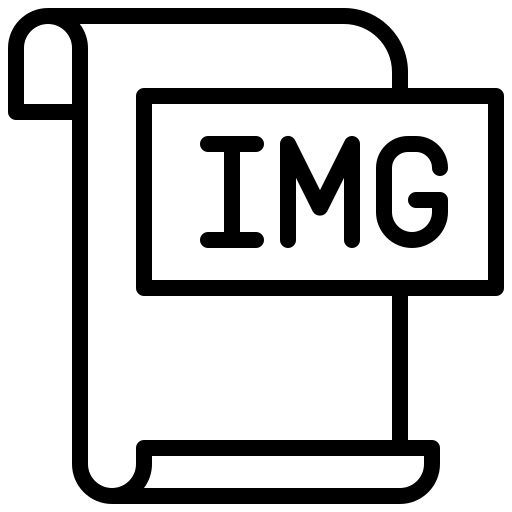
\includegraphics[width=0.5\textwidth]{img}
  \end{center}
  \caption{Imagem aleatória em .PNG}\label{fig:img}
\end{figure}


% --------------------------------------------- %

% --------------------------------------------- %
\end{document}
